\documentclass[a4paper,twoside]{ctexart}
\usepackage[xetex,bookmarks]{hyperref}
%\usepackage{BUPTthesisBachelor}
%网上说的将文献以上标形式出现,成功,可选参数有好几个,没记住...
\makeatletter
\def\@cite#1#2{\textsuperscript{[{#1\if@tempswa , #2\fi}]}}
\makeatother
\usepackage[top=1in, bottom=1in, left=1in, right=1in]{geometry}
\usepackage[xetex]{color,graphicx}

\CTEXoptions[today=big,contentsname={目\qquad 录},bibname={\textbf\heiti\zihao{3}参考文献}]
\CTEXsetup[format={\heiti\zihao{4}\bfseries\raggedright}]{section}
\CTEXindent

\setlength{\baselineskip}{20pt}  %设置行间距



\pagestyle{empty}
\begin{document}
\songti\zihao{4}
	\begin{center}
		\textsl{事件相关电位(ERPs)}无线同步协议设计与系统实现

		专业:通信工程\quad 班级:06123 \quad 学生姓名:樊高峰

		指导教师:洪波\quad 职称:副教授
	\end{center}
\noindent
\zihao{-4}
{\bfseries\heiti 摘要}

\songti
事件相关电位(Event-Related Potentials)是与刺激信号锁定的脑电信号的叠加平均。脑-机接口可以不依赖外围肌肉神经系统,实现人脑与外界直接通信。

事件相关电位的无线同步可以为基于事件相关电位的脑-机接口系统的应用提供灵活、便携性,同步采用子钟对准方案。三次握手完成无线同步触发器和脑电放大器同步计时。纠正后的两子钟计时偏差每小时小于1毫秒。系统精度为0.1毫秒,基于STM32实现。

\noindent {\bfseries\heiti 关键词} \quad 事件相关电位 \quad 无线同步 \quad 脑机接口

\noindent {\heiti\bfseries ABSTRACT}

The Event Related Potentials (ERPs) techniques average the EEG signals after the presentation of the stimulus through many trials to get the ERPs.As the stimulus synchronized ERPs was utilized in Brain Computer Interface which designs toward~\cite{Allison2007} people who suffer from severe neuromuscular disorders, a wireless connection would be efficient and flexible for daily applications.

This thesis designs and implements the wireless synchronization of ERP with the core idea of sub-clock synchronization. A 3-times Handshakes Process was designed to synchronize the device Wireless Trigger and Wireless EEG Amplifier. The difference between the two sub-clocks was less than 1 ms in a continuous recording of 60 minutes. The Wireless Trigger has a minimal time interval of $100 \mu s$ and was implemented in STM32 microprocessor.

\noindent {\heiti \bfseries KEY WORDS} \quad Event-Related Potentials\quad Wireless Synchronization \quad Brain Computer Interface
\section{引言-课题背景与意义}
事件相关电位(Event Related Potentials-ERPs)是一种脑电信号,它与刺激事件有严格的锁时关系,能提供其他脑活动记录方式(如fMRI)所没有的精确时域信息,被广泛运用在心理学和神经科学等领域。

脑电记录~\cite{LuckAugust12005}主要是通过被试(或用户)佩戴电极帽来完成,电极帽上每个电极(或者称为导联)的脑电信号经过放大,滤波和模数转换后以数字波形存储。如果在记录脑电的同时给被试以刺激(比如视觉刺激),与刺激时刻同步的脑电数据经叠加平均后就得到事件相关电位。基于事件相关电位的脑-机接口系统根据目标试次的事件相关电位与非目标试次事件相关电位的不同,利用模式识别的方法可以实现人脑与外界的直接通信,而不依赖于脊髓/外周肌肉神经系统。该技术为严重残障人士和运动神经损伤病人重建运动控制和恢复交流能力提供了可能~\cite{Wolpaw2000}。

这种日趋成熟的技术在应用方面还需要改进。无线的数据传输可以为该类应用提供灵活性和便携性。由于目前还没有为事件相关电位的刺激事件和脑电的无线同步提出解决方案~\cite{Chumerin2009}\cite{Lin2008}~\cite{Xu2009},本毕设的工作创新性地实现了事件相关电位的无线同步。

\textbf{方法 篇}主要介绍了事件相关电位无线同步的方案的设计和具体实现,\textbf{结果 篇}给出与系统性能相关的两个结果, \textbf{讨论 篇}探讨了实现中遇到的问题和改进。
\section{方法-同步协议与无线同步触发器实现}
提出两套实现事件相关电位无线同步的方案。方案一是蓝牙等间隔传输;该方案对于蓝牙延迟波动敏感,由于无线传输有$\pm 15 ms$的波动,最后被放弃。最终实现的是基于子钟对准硬同步的方案二。图~\ref{WirelessTriggerSche} 所示为方案二原理图。相比于有线系统,无线信道无法实时传输刺激事件。为实现事件相关电位的无线同步,在系统中增加了无线同步触发器(Wireless Trigger),该设备记录刺激事件发生的时刻,同时也接收无线脑电放大器发送的带有时间戳的脑电数据,因此只要实现无线同步触发器和无线脑电放大器的计时同步,就可以实现刺激事件和脑电数据的同步。

\begin{figure}[!hbp]
\begin{center}
\includegraphics[width=\textwidth]{graphic/SubClockWirelessSch.PNG} 
\caption{ 子钟对准硬同步原理框图 \label{WirelessTriggerSche}}
{\zihao{5}
[左上角为刺激屏幕,刺激范式为Odd-Ball范式,刺激矩阵以行或者列的方式随机闪烁,实验被试观察矩阵时的脑电数据被记录下来,对于被试想表达的字母或数字所在的行或者列闪烁得到的试次的事件相关电位与其他非目标行或列闪烁得到的事件相关电位信号在成分幅度和潜伏期上的差异可以通过模式识别的方法(比如支持向量机)加以判别,实现通信。]}
\end{center}
\end{figure}

\textbf{系统实现如下:}

在初始阶段通过三次握手完成无线同步触发器和无线脑电放大器子钟的同步计时。两系统将各自的一个输入管脚接到对方的一个输出管脚,并共地连接。三个管脚连接完成后进行握手确认。一次确认的过程是一方将其输出管脚电平做翻转,随后另一方在检测到这个电平翻转之后也将己方输出管脚电平做翻转以回应,完成双方的一次握手。三次握手之后,其中一方再给出一个电平翻转,两系统在该时刻同时使能内部的同步计时器,以0.1ms每次做递增,完成初始同步。

此后需要建立脑电数据与同步计数值之间的对应关系。脑电放大器以包的形式发送脑电数据给无线同步触发器,每个数据包都有一个帧号,并包含一段时间的脑电数据。以40ms一个数据包为例,规定从同步之后的第一个数据包开始,帧号从0x00到0xFF做循环。由于同步计数值以0.1ms每次做递增,帧号为0x01的第二个数据包就对应同步计数值400到799。无线同步触发器通过其内部计数(非同步计数值)保证循环后的帧号与同步计数值有正确的对应关系。

刺激事件信号存放在脑电数据采样点后增加的通道内。脑电数据按照导联(或称为电极)存储,对于模数转换器(ADC)精度为32bit的脑电放大器,一个导联的数据为4bytes。由于电极帽上通常不止一个电极,因此每个采样点的导联数也不为1。为了数据格式的兼容性,所以在每个采样点的导联之后增加一个空导联的字节数以存放刺激事件码。如果每采样点两电极记录,那么数据段每$2 \times 4 $bytes之后增加4bytes空间存放刺激事件码。

具体刺激事件信号属于那个采样点由该包的帧号,包采样时间和包采样点数决定(等同于采样率)。假设在同步计数值为659时有一个刺激事件,对于帧号为0x01(16进制的1),包采样时间为40ms,采样点数为4(等同于采样率100Hz)的脑电数据包。\textit{确定该刺激事件对应采样点位置}过程如下:
\begin{enumerate}
\item	根据帧号0x01和包的采样时间40ms,得出对应的同步计数值范围为400~799;
\item	由$400 < 659 < 799$,得到该刺激事件发生在该包采样时间段内;
\item 	根据采样点数4得出每个采样点对应的同步计数值个数:$400\div 4 = 100$;
\item 	将刺激事件对应的同步计数值减去该包计数范围的初始值:$659-400 = 259$;
\item 	将(4)计算结果除以(3)计算结果:$259\div 100 = 2 $余 $59$
\item 	确定该刺激事件为该包内按时间顺序的第$2+1$个采样点。
\end{enumerate}

记录刺激呈现第一个时刻的同步计数值作为该刺激事件的时刻。刺激呈现同时计算机通过并口给出高电平作为刺激事件码提供给无线同步触发器。\textit{一个典型的有效时间为15ms的高电平刺激事件信号只能被识别为一个刺激信号的处理}如下:
\begin{enumerate}
\item 	上电时,初始化上一次读取到有效电平时的同步计数值为0(PreCounter= 0);
\item 	检测是否有并口刺激事件信号;是则下一步,否则跳到6;
\item 	当前同步计数值(CurrCounter)是否等于PreCounter + 1?不是则下一步,是则跳转到6;
\item 	将当前同步计数值CurrCounter赋值给PreCounter;
\item 	保存该同步计数值CurrCounter作为刺激事件信号同步计数值;
\item 	结束,下一次进入时直接从(2)开始;
\end{enumerate}
该流程保证15ms刺激信号出现过程中,只有第一次计数值被记录,其后值都被忽略。

\section{结果-无线传输波动与子钟同步偏差}
\begin{itemize}
\item 
{\bfseries 无线传输波动(标准差):}
测试得到的蓝牙无线传输延迟波动为$\pm 15 ms$,证明方案一不可行。在两块同样的BTM0704串口蓝牙模块间进行测试,示波器分别监视发送和接收蓝牙的串口数据流。发端蓝牙发送等间隔的数据,接收端蓝牙接收。由于无线信道存在,如图~\ref{BTStaDeviation} 所示,无法做到蓝牙等间隔接收,方案一被否定。
\item
\textbf{子钟同步偏差:}
两子钟同步计数值的偏差随时间增长呈线性,纠正后偏差小于每小时1ms。事件相关电位无线同步方案二的关键就是无线同步触发器和无线脑电放大器子钟的计时同步,由于两系统晶振不同会导致计时偏差。令两系统的同步计数值除以10000的余数为1时翻转某一个管脚的输出电平,即当同步计数值为1,10001,20001,30001...时电平翻转,通过示波器监视这两个管脚的电平翻转情况,得到的两子钟随时间增长的计时偏差,如图~\ref{Difference} ,从上往下的三条曲线是无纠正时偏差,曲线拟合度大于0.99,平均斜率为171.1us/min。在经过100us/min和150us/min的纠正以后,如图中下两条曲线,偏差明显减小,其中150us/min纠正数据纵轴取值近0,达到计时偏差小于1ms/hour。
\end{itemize}

\begin{figure}[!hbp]
\begin{center}
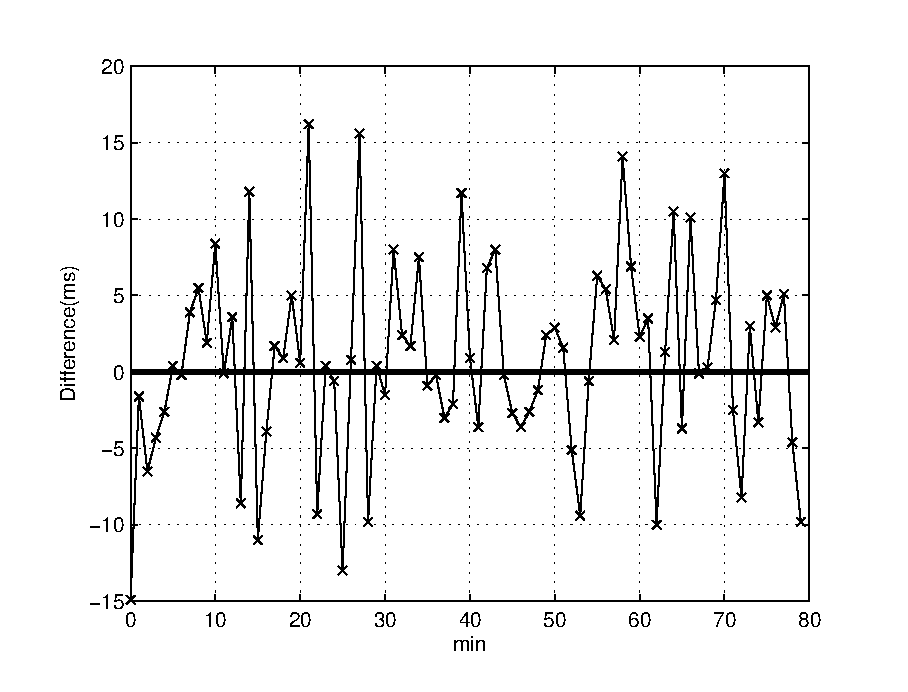
\includegraphics[width=0.9\textwidth]{graphic/equalSendBlueTooth.eps} 
\caption{蓝牙等间隔无线传输结果 \label{BTStaDeviation}}
{\zihao{5}
[横轴为某一次测试时间,纵轴为实际蓝牙接收间隔减去蓝牙数据发送间隔,由于发送间隔恒定,理想等间隔接收时间应等于发送时间,如图中粗线所示,实际数据表明蓝牙传输标准差在$\pm 15 ms$范围]}
\end{center}
\end{figure}

\begin{figure}[!hbp]
\begin{center}
\includegraphics[width=\textwidth]{graphic/PiezoOscillatorDifference.PNG} 
\caption{同步计数对准偏差 \label{Difference}}
\end{center}
\end{figure}
\section{讨论-问题与改进}
\begin{enumerate}
\item 如果无线同步触发器发往计算机的数据包大于1024bytes,数据段就会出错,但数据包小于1024bytes时,数据发送正常。上述操作代码相同,分配的空间足够,目前未找到原因,由于阈值刚好是1KB,考虑是否与系统缓存有关。
\item 刺激事件传输以并口的方式进行,考虑在下一步的系统实现中实现USB的刺激事件传输。
\end{enumerate}
\section{致谢}
感谢清华大学医学院神经工程实验室的洪波副教授和博士生胥红来对于我毕设工作的指导和支持,感谢北京邮电大学对于我的培养和帮助,使我能顺利完成该校外毕设任务。

\CTEXsetup[format+={\centering}]{section}

{\songti\zihao{5}
\bibliographystyle{IEEEtran}
\bibliography{IEEEabrv,ref/referenceUndergraduate}
}

\end{document}
